\documentclass[11pt]{amsart}
\usepackage{geometry}                % See geometry.pdf to learn the layout options. There are lots.
\geometry{letterpaper}                   % ... or a4paper or a5paper or ... 
%\geometry{landscape}                % Activate for for rotated page geometry
%\usepackage[parfill]{parskip}    % Activate to begin paragraphs with an empty line rather than an indent
\usepackage{graphicx}
\usepackage{amssymb}
\usepackage{epstopdf}
\usepackage{amsmath}
\usepackage{tikz}

\DeclareGraphicsRule{.tif}{png}{.png}{`convert #1 `dirname #1`/`basename #1 .tif`.png}
\usetikzlibrary{arrows,positioning}
% LB things
\newenvironment{packed_item}{
\begin{itemize}
 \setlength{\itemsep}{0pt}
  \setlength{\parskip}{0pt}
  \setlength{\parsep}{0pt}
}{\end{itemize}}

\newcommand{\Unif}{\text{Unif}}
\newcommand{\Beta}{\text{Beta}}
\newcommand{\Normal}{\text{Normal}}
\newcommand{\Binomial}{\text{Binomial}}
\newcommand{\E}{\mathbb{E}}
 
 




\title{Mechanistic Bayesian Forecasts of COVID19}
\author{Graham Gibson}
%\date{}                                           % Activate to display a given date or no date


\begin{document}
\section*{Abstract}
\begin{itemize}
\item Covid has affected XX people
\item Forecasts useful for public health resource planning, intervention planning (vaccine trials), and disease burden
\item Basic Mechanistic Models unable to capture complexities of real world disease epidemics due to 
\begin{itemize}
\item Complexities of interventions 
\item Issues with testing and reporting
\end{itemize}
\item We propose a novel forecasting algorithm to overcome 
\begin{itemize}
\item Under-reporting of cases
\item Time-varying interventions
\end{itemize}
\item Bayesian end to end estimation using both cases and deaths in numpyro
\end{itemize}


\maketitle

%\section{}
%\subsection{}

\section{Introduction}

\begin{itemize}
\item Emergence and spread of covid
\item Forecasts useful for public health
\begin{itemize}
\item Resource allocation
\item Intervention Planning
\item Disease burden
\end{itemize}
\item Cite Flu Forecasting
\item Describe COVID-HUB
\begin{itemize}
\item Number of participating teams as evidence of importance
\item Soliciting forecasts for incident and cumulative deaths
\end{itemize}
\item Mechanistic models have been around since K\&K
\item Demonstrated success in modeling infectious disease 
\item Since they were developed around the last pandemic their usefulness as applied forecasting models has gone untested
\item Extensions to basic model needed 
\begin{itemize}
\item Observations on cases and deaths
\item Time-varying detection probability for varied testing
\item Non-parametric model of interventions
\item Full Bayesian fitting due to unidentifiability of parameters given only a time series of cases and deaths.
\end{itemize}
\item MechBayes outperforms in two settings
\begin{itemize}
\item COVID-HUB relative to baseline model 
\item Ablation test relative to basic SEIR model
\end{itemize}
\item We show improvements in MAE and WIS relative to baseline model in both experimental setups

\end{itemize}

\section{Data}

\begin{itemize}
\item We use cases/deaths from JHU
\item Under-reporting issues
\item Batch reporting issues
\item Revision Issues
\item Weekly cycle issues
\item High variability in incident data
\item Ref Figure 1
\end{itemize}





 \begin{figure}
     \centering
     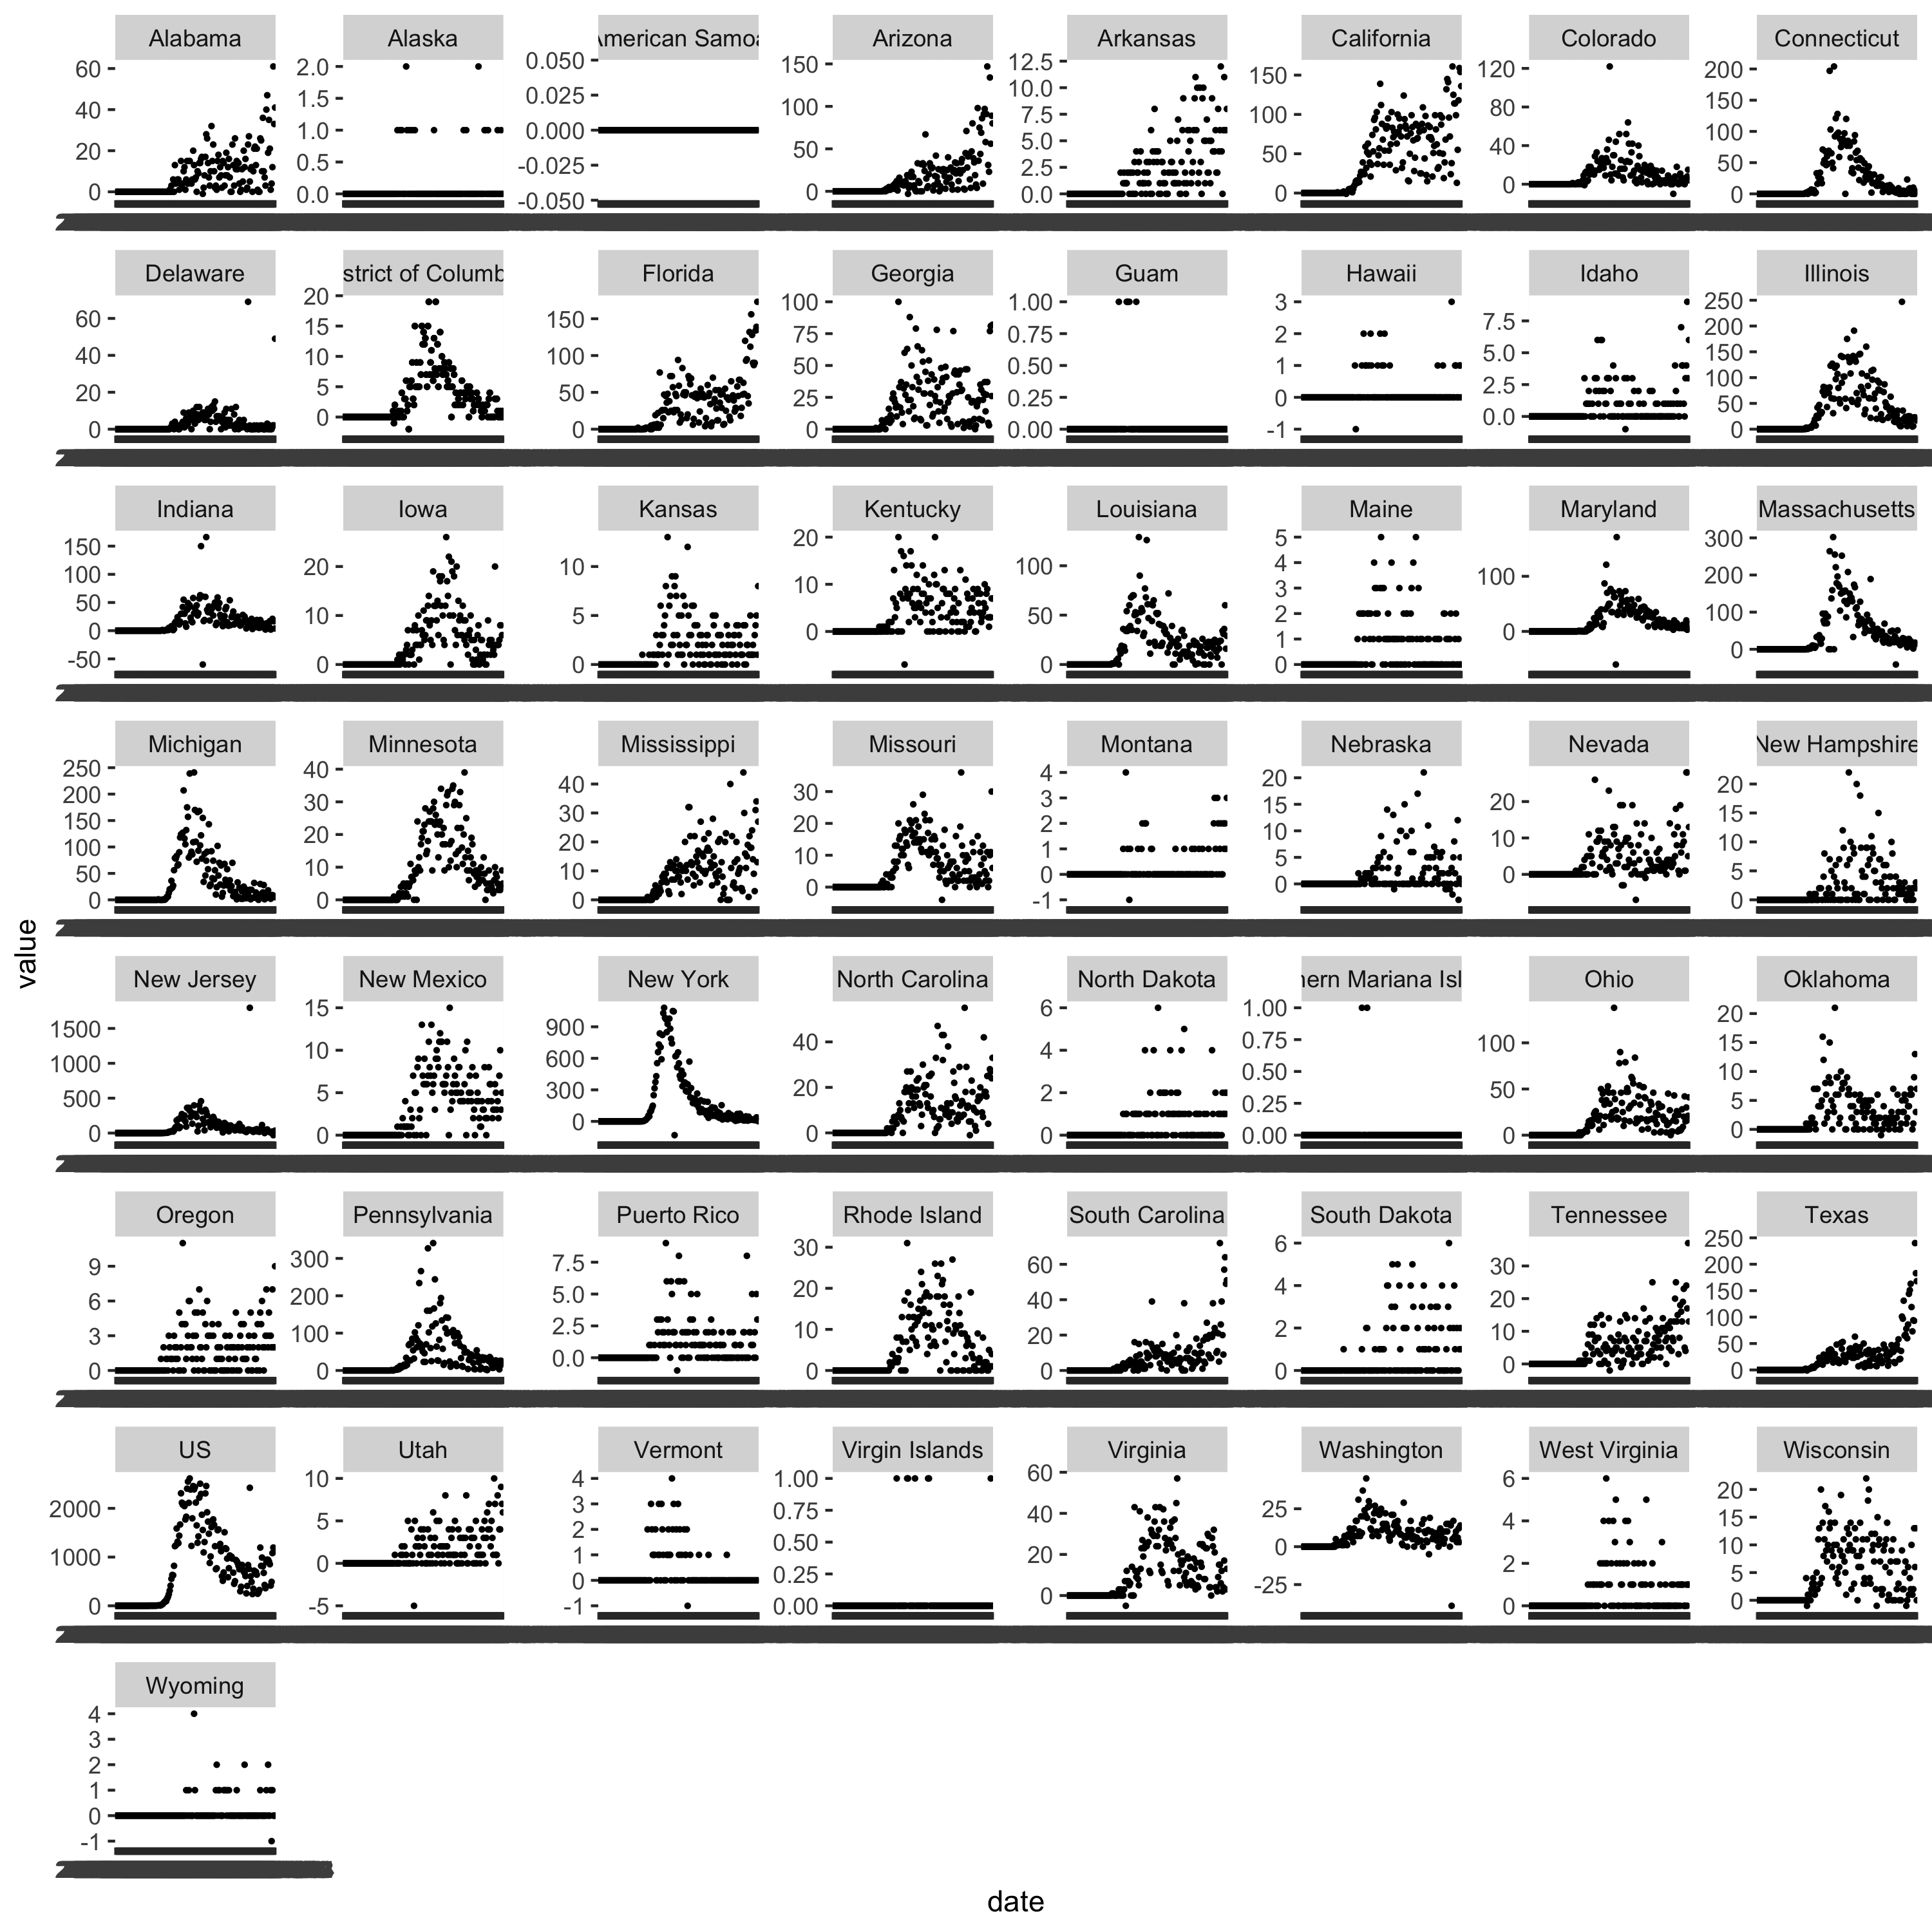
\includegraphics[scale=.1]{data_plot.png}
     \caption{Deaths by state. }
     \label{fig:my_label}
 \end{figure}
 
 \section{Compartmental Model}
 \begin{itemize}
 \item Basic SEIR model description
 \item Definition of compartmental model (description of diff eq as flow between compartments)
 \item Ref Figure 2
 \item Interpretation of parameters in basic SEIR model 
 \begin{itemize}
 \item Sigma
 \item Gamma
 \item beta
 \end{itemize}
 
 \end{itemize}
 
 \begin{figure}
     

 \begin{center}
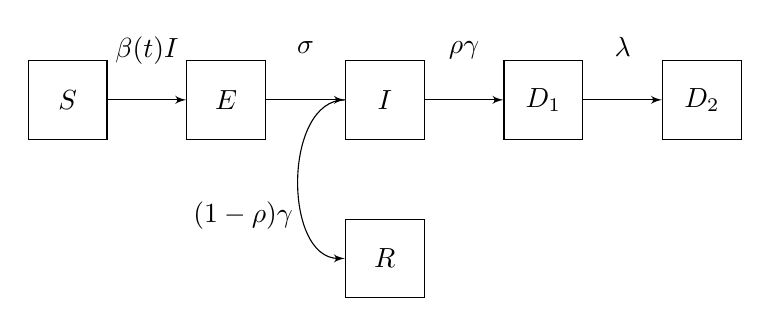
\begin{tikzpicture}[node distance=1cm,auto,>=latex',every node/.append style={align=center},int/.style={draw, minimum size=1cm}]
    \node [int] (S)             {$S$};
      \node [int,right=of S] (E)  {$E$};
    \node [int, right=of E] (I) {$I$};
    \node [int, right=of I] (D_1) {$D_1$};
    \node [int, right=of D_1] (D_2) {$D_2$};
     \node [int, below=of I] (R) {$R$};

   % \coordinate[right=of ] (out); %
    \path[->, auto=false] (S) edge node[yshift=12pt] {$\beta(t) I$ \\[.2em]} (E)
                          (E) edge node[yshift=12pt] {$\sigma$       \\[.2em] } (I) 
                           (I) edge node[yshift=12pt] {$\rho\gamma$       \\[.2em] } (D_1)
                           (I) edge[bend right=90] node[xshift=-20pt,yshift=-20pt] {$(1-\rho)\gamma$       \\[.4em] } (R)
                            (D_1) edge node[yshift=12pt] {$\lambda$       \\[.2em] } (D_2)  ;
                          \end{tikzpicture}
\end{center}
      \caption{Comparmental model parameters }
     \label{fig:seird}
 \end{figure}
 \subsection{Observations on cases and deaths}
 \begin{itemize}
 \item Bayesian model has observations on both cases and deaths
 \item We can weight likelihood of one over the other
 \item Explain how cases inform deaths on average 10 days later
 \end{itemize}
 
 \subsection{Time-varying beta parameter}
 \begin{itemize}
 \item Non-parametrically models time-varying transmissibility through a random walk
 \item Makes forecasts conditional on current level of interventions
 \item Requires no external intervention data to make forecasts 
 \item 
 \end{itemize}
 
 \subsection{Time-varying detection probability}
  \begin{itemize}
 \item Non-parametrically models time varying testing and overall detection of case issues
 \item Allows for "data dumps"
 \item Logistic random walk 
 \item Fixed detection probability on deaths

  \end{itemize}

\subsection{Seeding Epidemic}

 \begin{itemize}
 \item Because of detection probability we cannot seed using initial reported data, since this is an underestimate
  \end{itemize}

\end{document}  